\documentclass[../main.tex]{subfiles}
\subsection{GPIO}
The function \emph{setupGPIO()} will be called in the main function to activate GPIO functionalities.
The implementation of the function is located in the /emph{setup.c} file.

\begin{minted}{objdump}
void setupGPIO()
{
/* enable GPIO clock*/
*CMU_HFPERCLKEN0 |= CMU2_HFPERCLKEN0_GPIO;
    
/* set high drive strength */
*GPIO_PA_CTRL = 2;  
    
/* set pins A8-15 as output */
*GPIO_PA_MODEH = 0x55555555; 
    
/* turn on LEDs D1-D8 (LEDs are active low) */
*GPIO_PA_DOUT = 0x0000; 
    
/* Set pins 0-7 */
*GPIO_PC_MODEL = 0x33333333; 
    
/* Enable internal pull-up */
*GPIO_PC_DOUT = 0xff; 
    
/* Write 0x22222222 to register */
*GPIO_EXTIPSELL = 0x22222222; 
    
/* Set interrupt on 1->0 transition */
*GPIO_EXTIFALL = 0xff; 
    
/* Enable interrupt generation */
*GPIO_IEN = 0xff; 
}
\end{minted}

After the GPIO setup is completed, when ever a button is pressed, the /emph{handle\_gpio()} function i s called and the desired code will be executed.

\begin{figure}
    \centering
    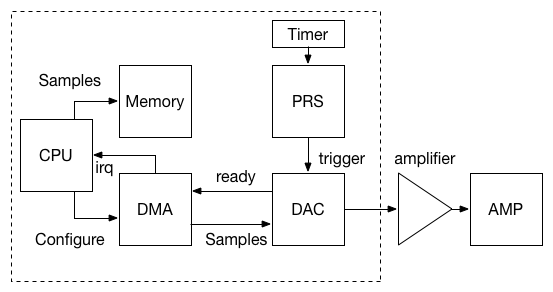
\includegraphics[width=0.4\textwidth]{fig/DMA-DAC.png}
    \caption{Overview of DMA-DAC system}
    \label{fig:DMA-DAC}
\end{figure}
